\documentclass[border=0pt]{standalone}
\usepackage{tikz}
\usetikzlibrary{positioning,shapes,arrows.meta,patterns,calc}
\definecolor{garnet}{HTML}{73000A}
\definecolor{coral}{HTML}{CC2E40}
\definecolor{slate}{HTML}{466A9F}
\definecolor{teal}{HTML}{1F414D}
\definecolor{olive}{HTML}{65780B}
\definecolor{lime}{HTML}{CED318}
\definecolor{gold}{HTML}{A49137}
\begin{document}
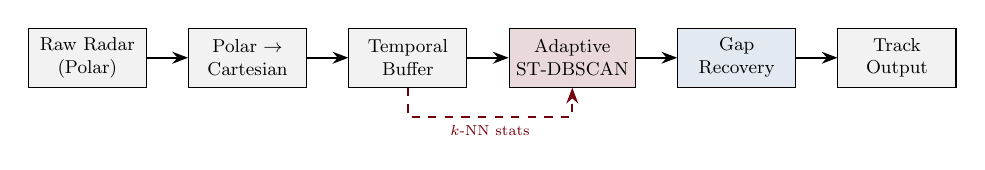
\begin{tikzpicture}[scale=0.75, transform shape,
    node distance=0.7cm,
    block/.style={rectangle, draw=black, fill=gray!10, minimum height=1cm, minimum width=2cm, align=center, font=\small},
    arrow/.style={-{Stealth[length=2mm]}, thick, draw=black}
]
    % Nodes
    \node[block] (raw) {Raw Radar\\(Polar)};
    \node[block, right=of raw] (cart) {Polar $\to$\\Cartesian};
    \node[block, right=of cart] (buffer) {Temporal\\Buffer};
    \node[block, right=of buffer, fill=garnet!15] (stdbscan) {Adaptive\\ST-DBSCAN};
    \node[block, right=of stdbscan, fill=slate!15] (gap) {Gap\\Recovery};
    \node[block, right=of gap] (tracks) {Track\\Output};
    
    % Arrows
    \draw[arrow] (raw) -- (cart);
    \draw[arrow] (cart) -- (buffer);
    \draw[arrow] (buffer) -- (stdbscan);
    \draw[arrow] (stdbscan) -- (gap);
    \draw[arrow] (gap) -- (tracks);
    
    % Feedback arrow for adaptive epsilon
    \draw[arrow, dashed, garnet] (buffer.south) -- ++(0,-0.5) -| node[pos=0.25, below, font=\scriptsize] {$k$-NN stats} (stdbscan.south);
\end{tikzpicture}
\end{document}
